\chapter{Results and Discussion}
\label{ch:results}

All numbers below are averaged over the 13 layers of the arXiv co-authorship network. Learning-based
models are reported as mean~$\pm$~standard deviation over five random seeds; classical heuristics are
deterministic and therefore have no spread.

\section{Overall Classification Performance}
Table~\ref{tab:overall} reports ROC-AUC, PR-AUC, and F1-score for every method, and
Figure~\ref{fig:roc} and Figure~\ref{fig:allmetrics} show the same results graphically. The
\textbf{proposed model attains the highest ROC-AUC} (0.873), narrowly ahead of the strong classical
heuristics and clearly ahead of the graph-neural baselines GAT (0.822) and GCN (0.767). Node2Vec
leads on PR-AUC and F1, and the classical heuristics lead on F1; this is discussed below.

\begin{table}[htbp]
\centering
\caption{Overall classification performance, averaged over the 13 layers. \emph{Std} is the standard
deviation of ROC-AUC over 5 random seeds; classical heuristics are deterministic (--). Best value per
column in bold.}
\label{tab:overall}
\renewcommand{\arraystretch}{1.25}
\begin{tabular}{lcccc}
\toprule
\textbf{Model} & \textbf{ROC-AUC} & \textbf{Std} & \textbf{PR-AUC} & \textbf{F1-score} \\
\midrule
Proposed A (ours)       & \textbf{0.873} & 0.001 & 0.893 & 0.814 \\
Proposed B (ours)       & 0.871 & 0.003 & 0.895 & 0.810 \\
Adamic--Adar            & 0.872 & --    & 0.872 & 0.850 \\
Jaccard                 & 0.872 & --    & 0.871 & 0.849 \\
Common Neighbours       & 0.872 & --    & 0.871 & 0.851 \\
Node2Vec                & 0.847 & 0.001 & \textbf{0.907} & \textbf{0.868} \\
GAT                     & 0.822 & 0.007 & 0.825 & 0.780 \\
GCN                     & 0.767 & 0.011 & 0.797 & 0.743 \\
Preferential Attachment & 0.603 & --    & 0.656 & 0.666 \\
\bottomrule
\end{tabular}
\end{table}

\begin{figure}[htbp]
\centering
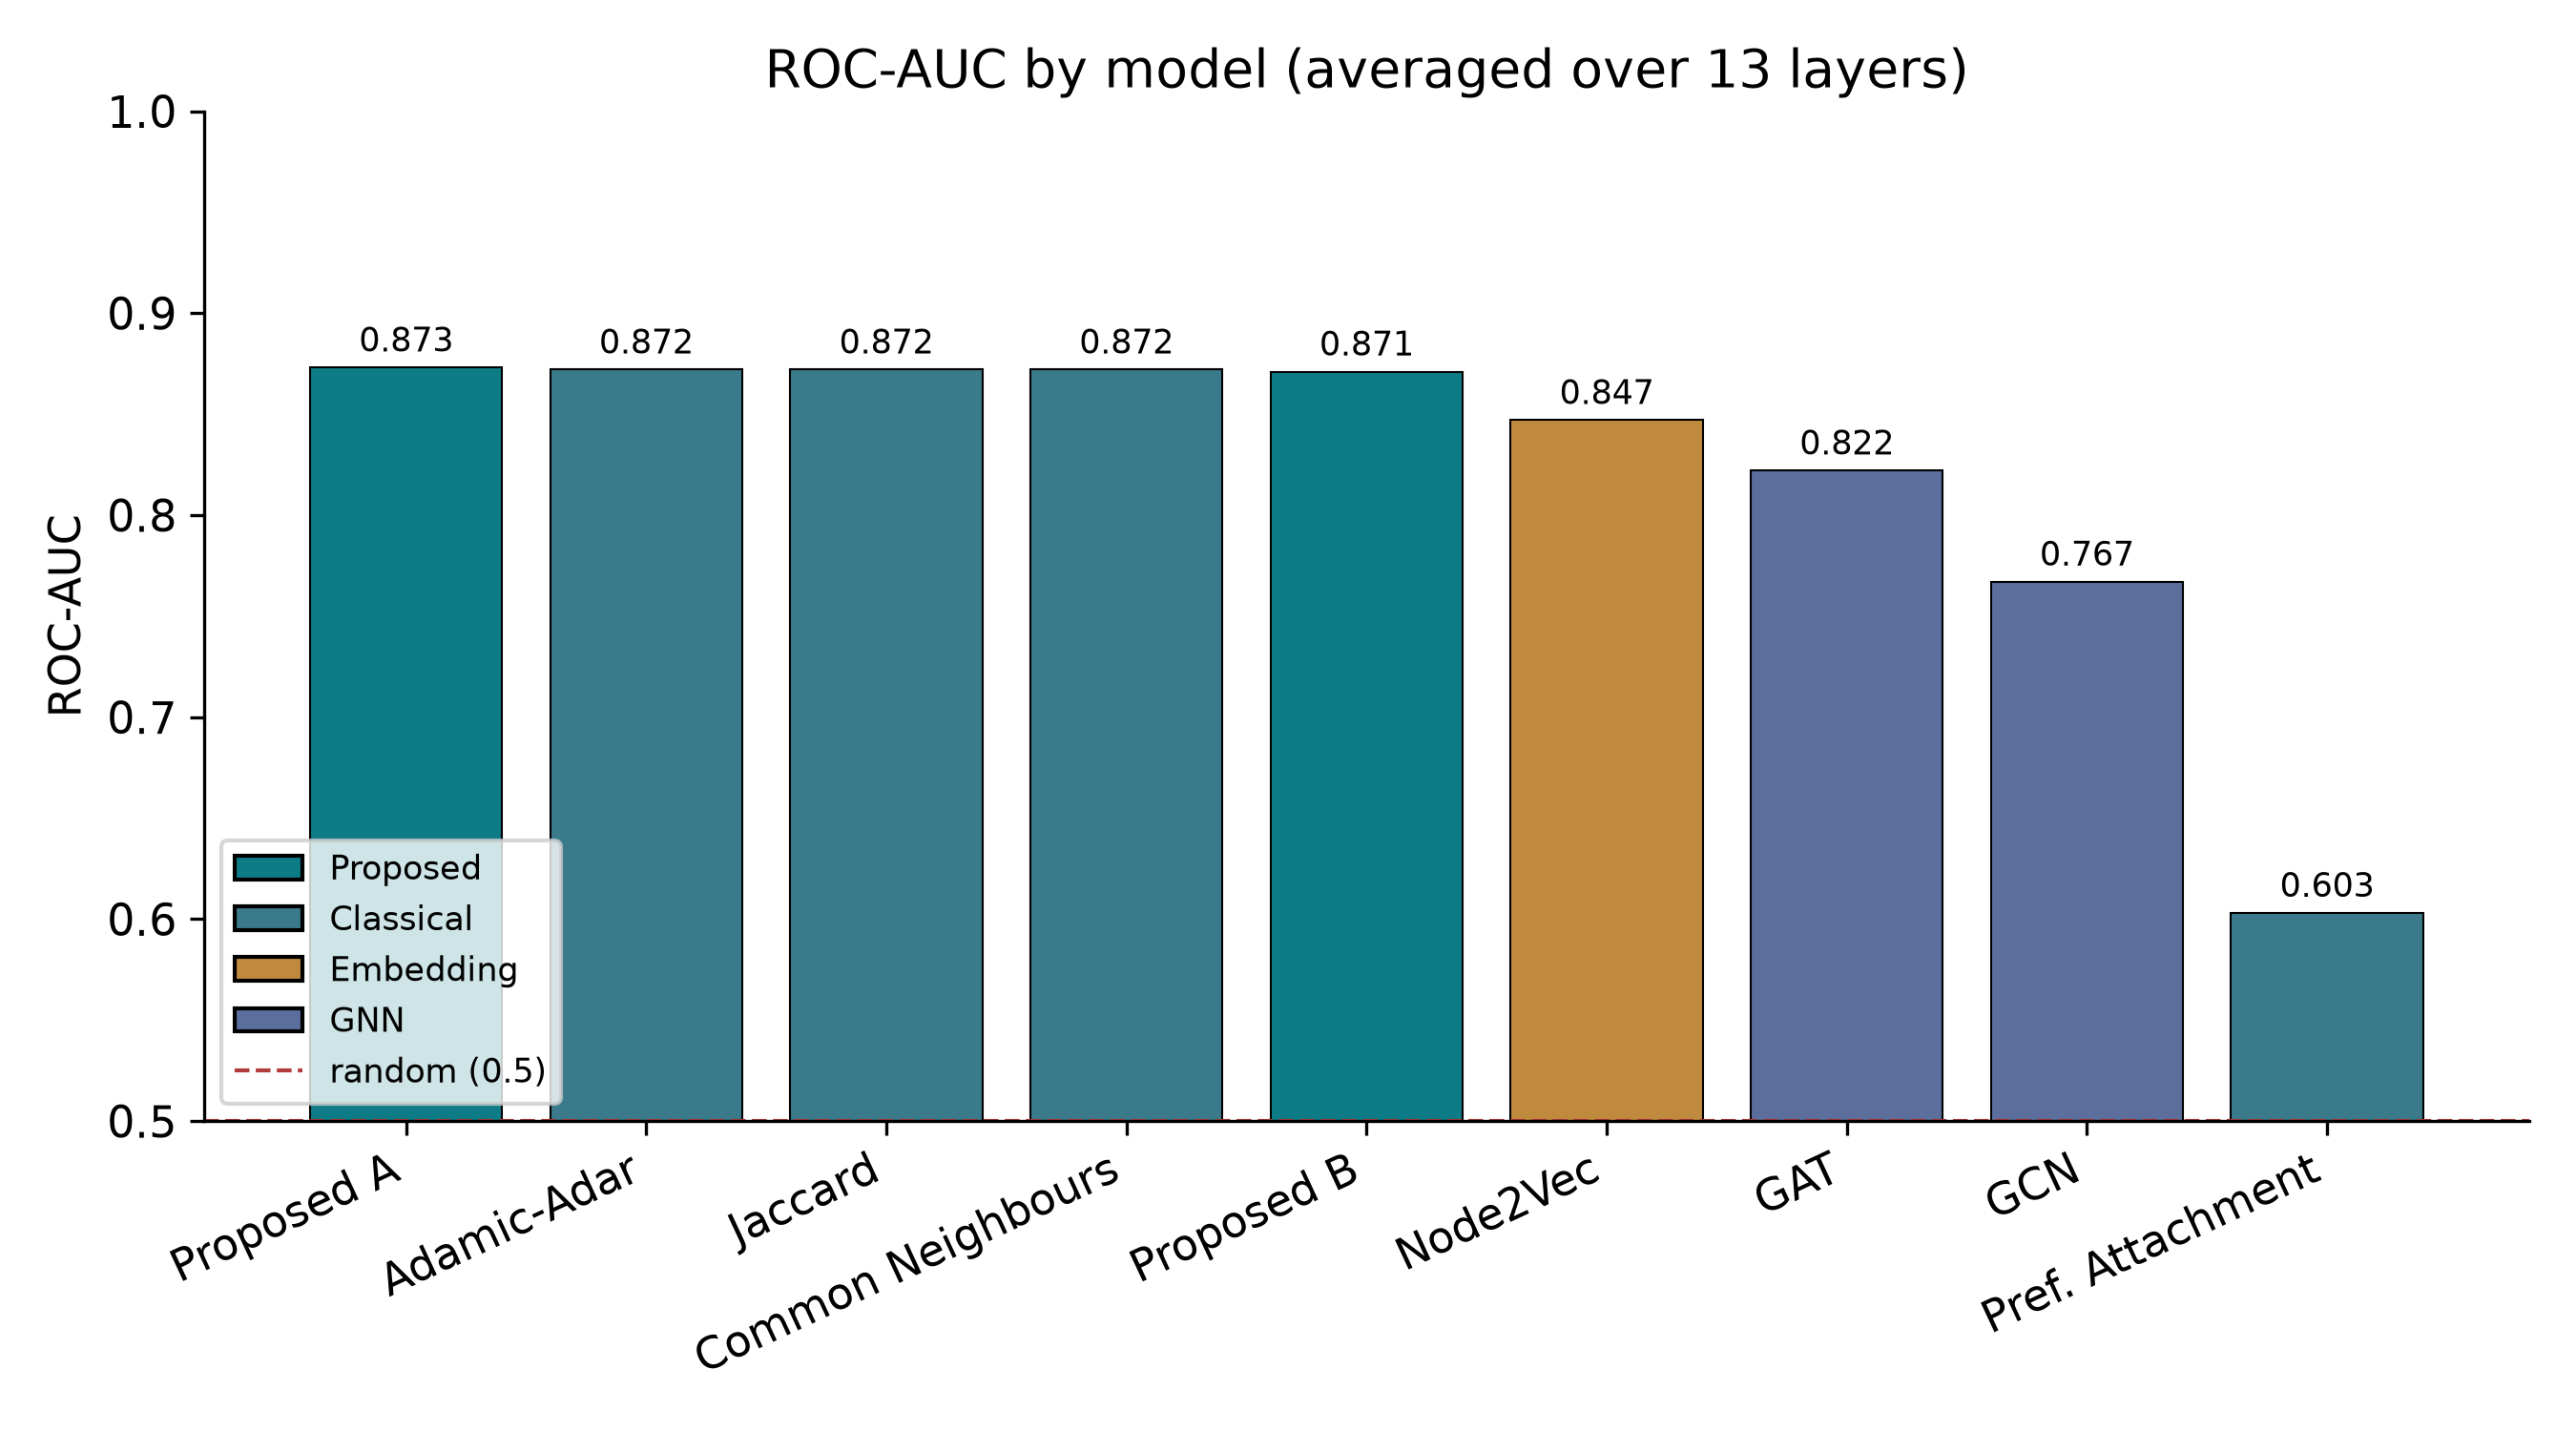
\includegraphics[width=0.9\textwidth]{figures/fig1_roc_auc.png}
\caption{ROC-AUC by model, averaged over the 13 layers. The dashed line marks random performance
(0.5). The proposed model attains the highest value.}
\label{fig:roc}
\end{figure}

\begin{figure}[htbp]
\centering
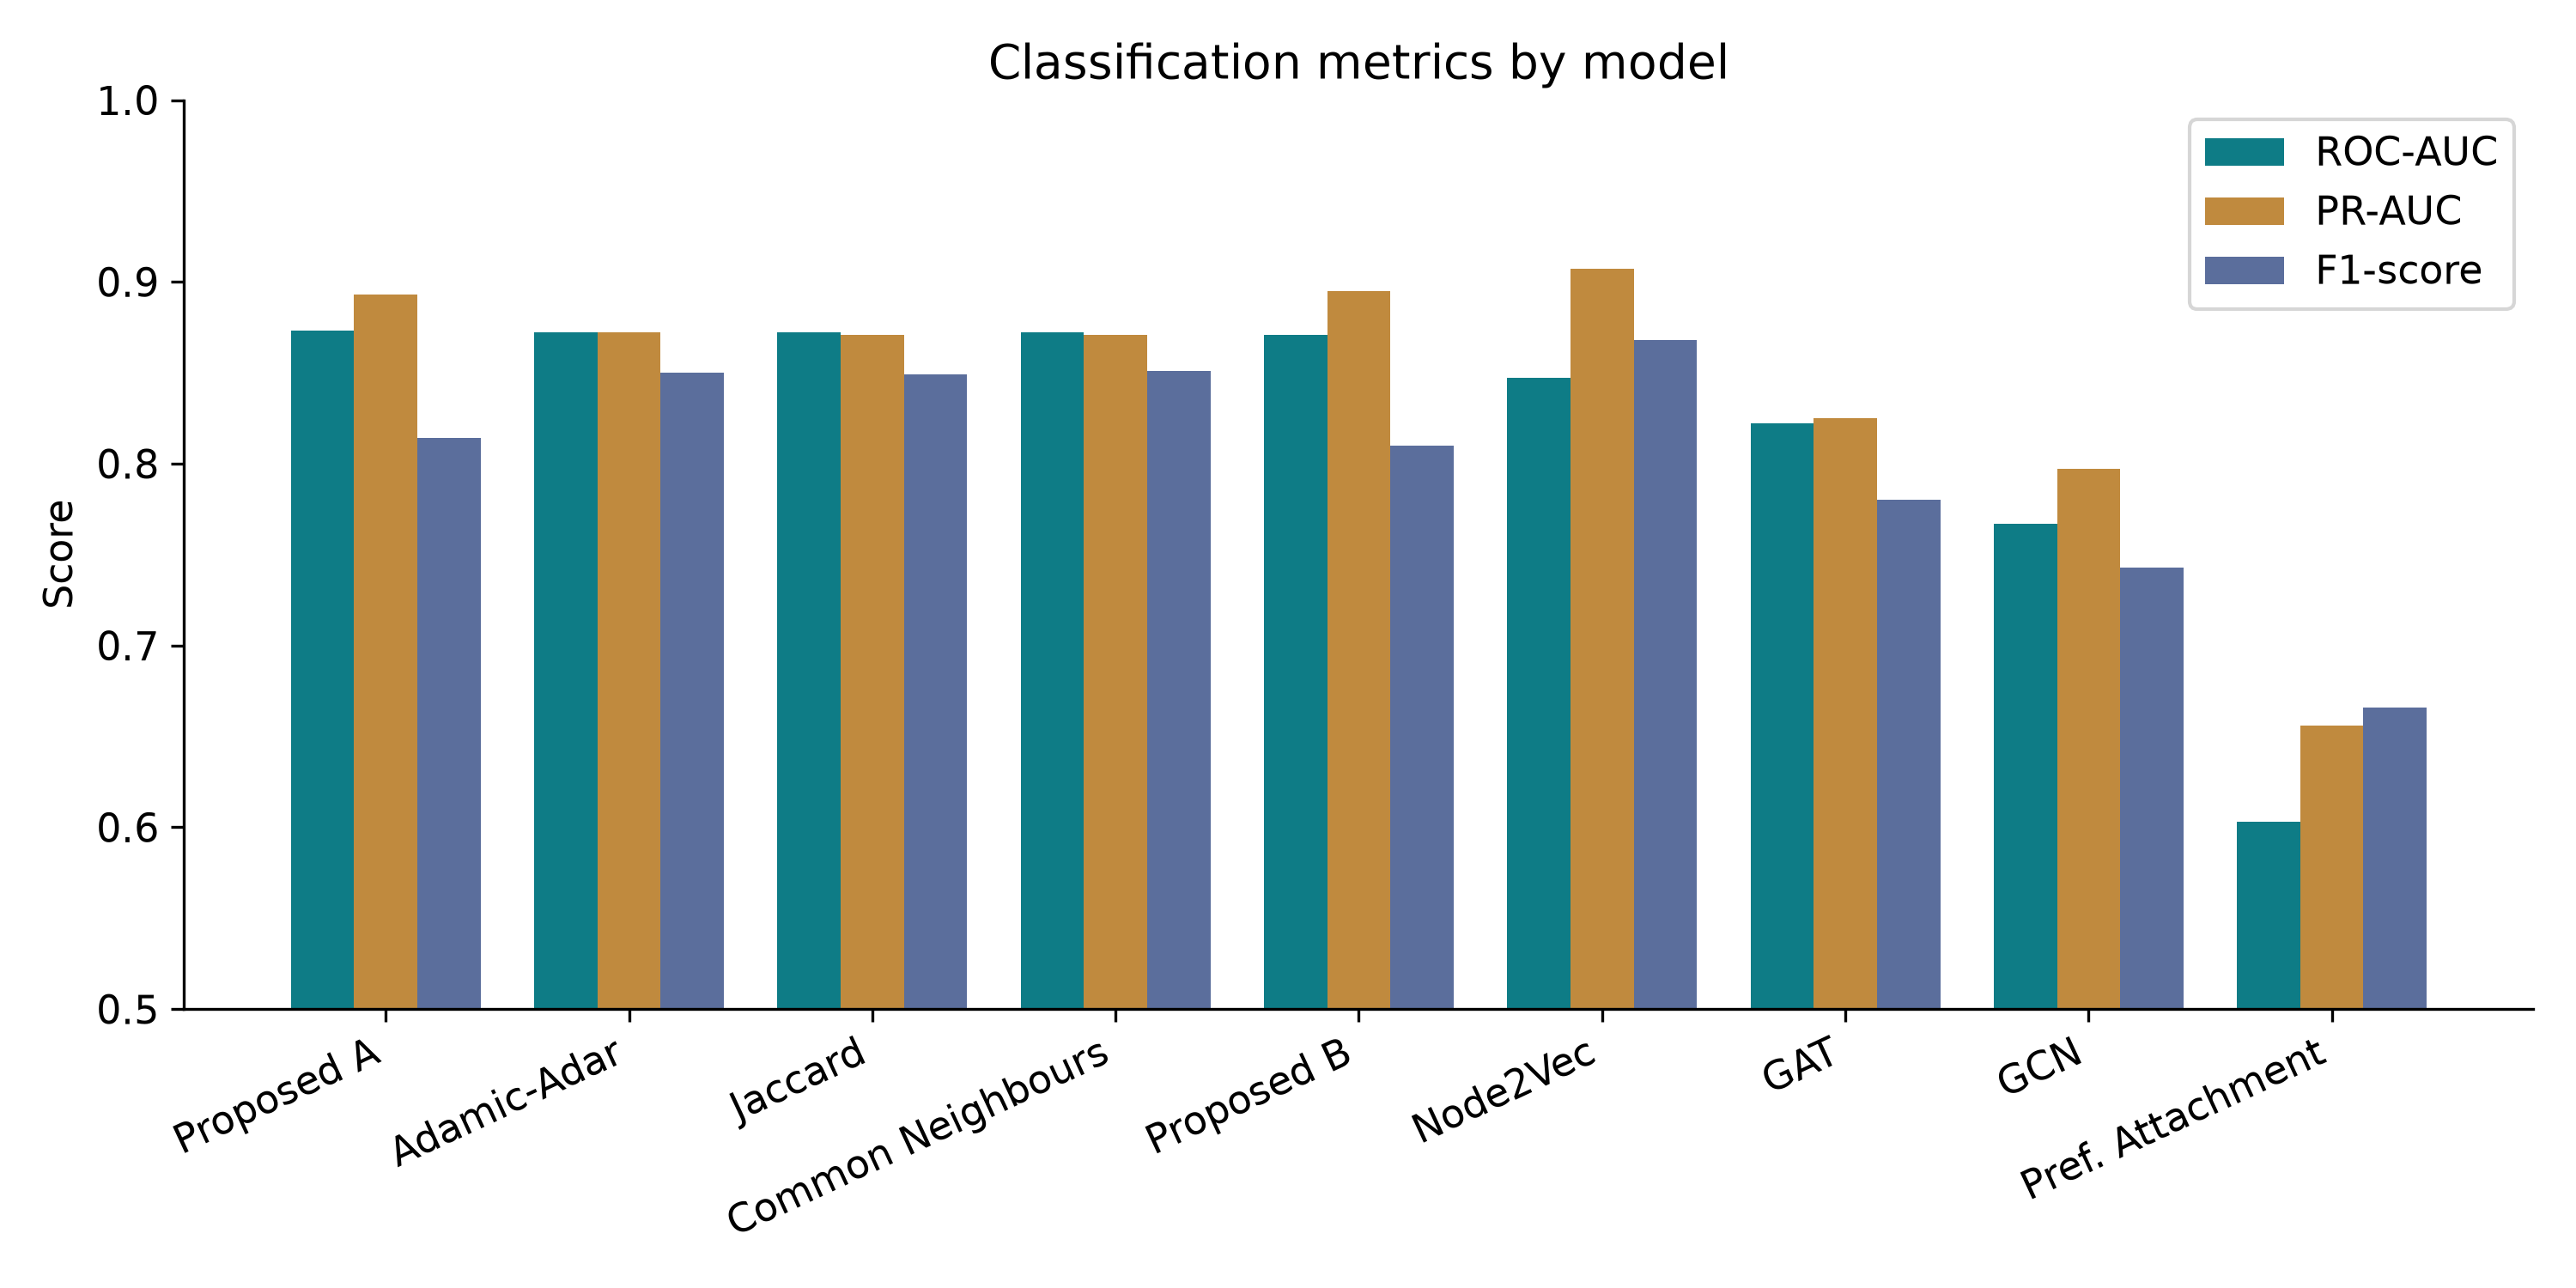
\includegraphics[width=0.95\textwidth]{figures/fig2_all_metrics.png}
\caption{ROC-AUC, PR-AUC, and F1-score side by side for all methods.}
\label{fig:allmetrics}
\end{figure}

\section{Statistical Significance}
Because several models are close on ROC-AUC, the improvement of the proposed model over the neural
baselines was tested with a paired $t$-test across the five seeds (Table~\ref{tab:signif}). The gains
over both GAT and GCN are \textbf{statistically significant} on all three metrics ($p<0.001$),
confirming that the improvement over the neural baselines is systematic rather than an artefact of a
lucky split.

\begin{table}[htbp]
\centering
\caption{Paired $t$-test of the proposed model against the neural baselines (5 seeds). $\Delta$ is
the mean improvement.}
\label{tab:signif}
\renewcommand{\arraystretch}{1.25}
\begin{tabular}{llcc}
\toprule
\textbf{Comparison} & \textbf{Metric} & \textbf{$\Delta$} & \textbf{$p$-value} \\
\midrule
Proposed A vs GAT & ROC-AUC & $+0.051$ & $8.9\times10^{-5}$ \\
Proposed A vs GCN & ROC-AUC & $+0.107$ & $3.3\times10^{-5}$ \\
Proposed A vs GAT & PR-AUC  & $+0.067$ & $1.1\times10^{-5}$ \\
Proposed A vs GCN & PR-AUC  & $+0.096$ & $3.4\times10^{-5}$ \\
Proposed A vs GAT & F1      & $+0.035$ & $1.1\times10^{-5}$ \\
Proposed A vs GCN & F1      & $+0.071$ & $5.5\times10^{-6}$ \\
\bottomrule
\end{tabular}
\end{table}

\section{Weak-Tie versus Common-Neighbour Links}
The central claim of this work is examined in Table~\ref{tab:weaktie} and Figure~\ref{fig:weaktie},
which split the test edges into \emph{weak-tie} links (endpoints sharing no neighbours) and
\emph{common-neighbour} links, and report ROC-AUC on each. The result is decisive: on weak-tie links
every classical heuristic scores exactly \textbf{0.500 -- pure chance} -- because their score is zero
whenever the shared-neighbour count is zero. The attention-based models are the only ones that rise
meaningfully above chance, with GAT (0.623) and the proposed model (0.615) leading. On
common-neighbour links the ordering reverses, with the classical heuristics strongest (up to 0.886).
The proposed model is the best \emph{all-rounder}: it is the only method that is both competitive on
weak-tie links and solid on common-neighbour links, whereas each other family is strong on one type
and weak on the other.

\begin{table}[htbp]
\centering
\caption{ROC-AUC on weak-tie links versus common-neighbour links. Classical heuristics are provably
random (0.500) on weak-tie links.}
\label{tab:weaktie}
\renewcommand{\arraystretch}{1.25}
\begin{tabular}{lcc}
\toprule
\textbf{Model} & \textbf{Weak-tie links} & \textbf{Common-neighbour links} \\
\midrule
GAT                     & \textbf{0.623} & 0.415 \\
Proposed A (ours)       & 0.615 & 0.493 \\
Proposed B (ours)       & 0.607 & 0.531 \\
Adamic--Adar            & 0.500 & \textbf{0.886} \\
Jaccard                 & 0.500 & 0.747 \\
Common Neighbours       & 0.500 & 0.716 \\
Node2Vec                & 0.434 & 0.679 \\
GCN                     & 0.433 & 0.576 \\
Preferential Attachment & 0.253 & 0.535 \\
\bottomrule
\end{tabular}
\end{table}

\begin{figure}[htbp]
\centering
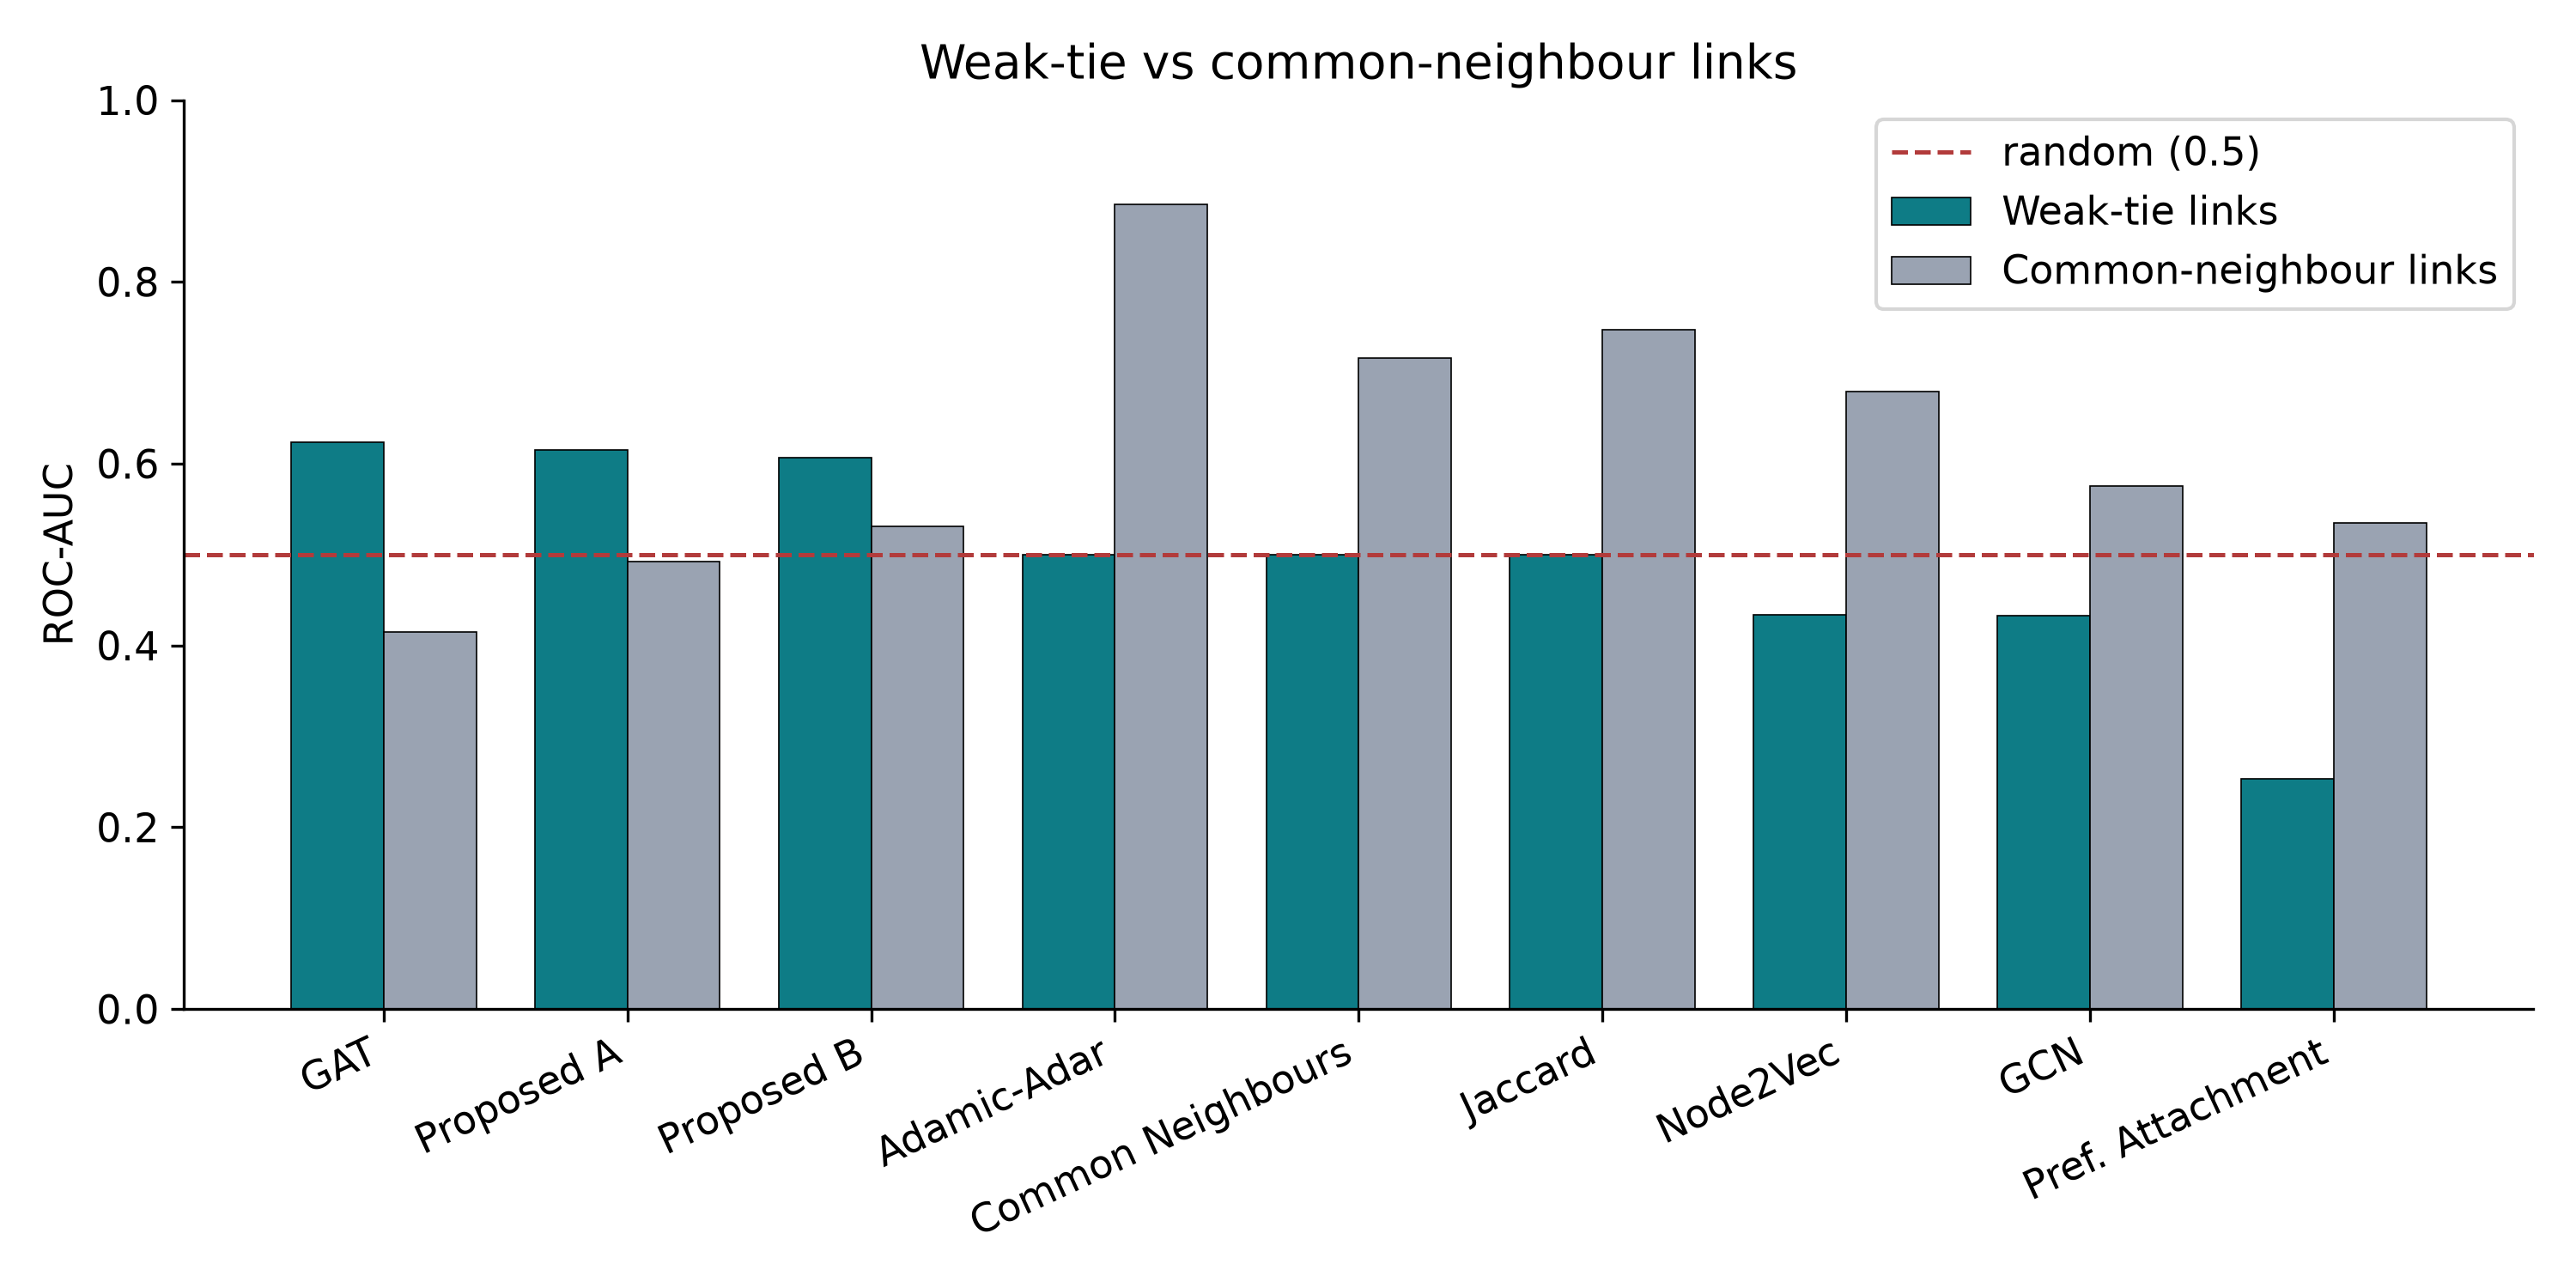
\includegraphics[width=0.95\textwidth]{figures/fig3_weaktie_vs_commonneighbour.png}
\caption{Weak-tie versus common-neighbour ROC-AUC. Only the attention-based models rise above the
random line (0.5) on weak-tie links; classical heuristics sit exactly on it.}
\label{fig:weaktie}
\end{figure}

\section{Ranking Performance}
Table~\ref{tab:ranking} reports the ranking metrics. Here the classical heuristic Adamic--Adar leads
(MRR~0.667), followed by the other neighbourhood methods and Node2Vec; the proposed model is mid-pack
on ranking. This is consistent with the previous section: ranking is dominated by the many
common-neighbour pairs, on which the heuristics excel. Ranking is therefore reported honestly as a
metric on which the proposed model does not lead, and improving it is left as future work.

\begin{table}[htbp]
\centering
\caption{Ranking performance (higher is better).}
\label{tab:ranking}
\renewcommand{\arraystretch}{1.25}
\begin{tabular}{lccccc}
\toprule
\textbf{Model} & \textbf{MRR} & \textbf{Hits@1} & \textbf{Hits@3} & \textbf{Hits@5} & \textbf{Hits@10} \\
\midrule
Adamic--Adar        & \textbf{0.667} & \textbf{0.590} & \textbf{0.730} & \textbf{0.739} & 0.746 \\
Jaccard             & 0.575 & 0.447 & 0.690 & 0.707 & 0.731 \\
Common Neighbours   & 0.559 & 0.388 & 0.678 & 0.724 & \textbf{0.746} \\
Node2Vec            & 0.507 & 0.395 & 0.591 & 0.646 & 0.730 \\
Proposed B (ours)   & 0.335 & 0.248 & 0.361 & 0.415 & 0.507 \\
Proposed A (ours)   & 0.283 & 0.196 & 0.312 & 0.371 & 0.473 \\
GCN                 & 0.149 & 0.091 & 0.157 & 0.186 & 0.257 \\
GAT                 & 0.144 & 0.081 & 0.143 & 0.190 & 0.274 \\
Preferential Attachment & 0.090 & 0.054 & 0.083 & 0.110 & 0.149 \\
\bottomrule
\end{tabular}
\end{table}

\section{Interpretability: Per-Layer Behaviour and Layer Importance}
A practical advantage of the model is that its cross-layer attention can be read back.
Figure~\ref{fig:heatmap} shows per-layer ROC-AUC across the 13 research domains, revealing which
domains are easy or hard for each method, and Figure~\ref{fig:beta} shows the learned
layer-importance weights $\beta_\ell$. These weights indicate which research domains the model relies
on most when combining evidence across layers, turning the model from a black box into an object that
can be inspected and explained -- something none of the baselines offer.

\begin{figure}[htbp]
\centering
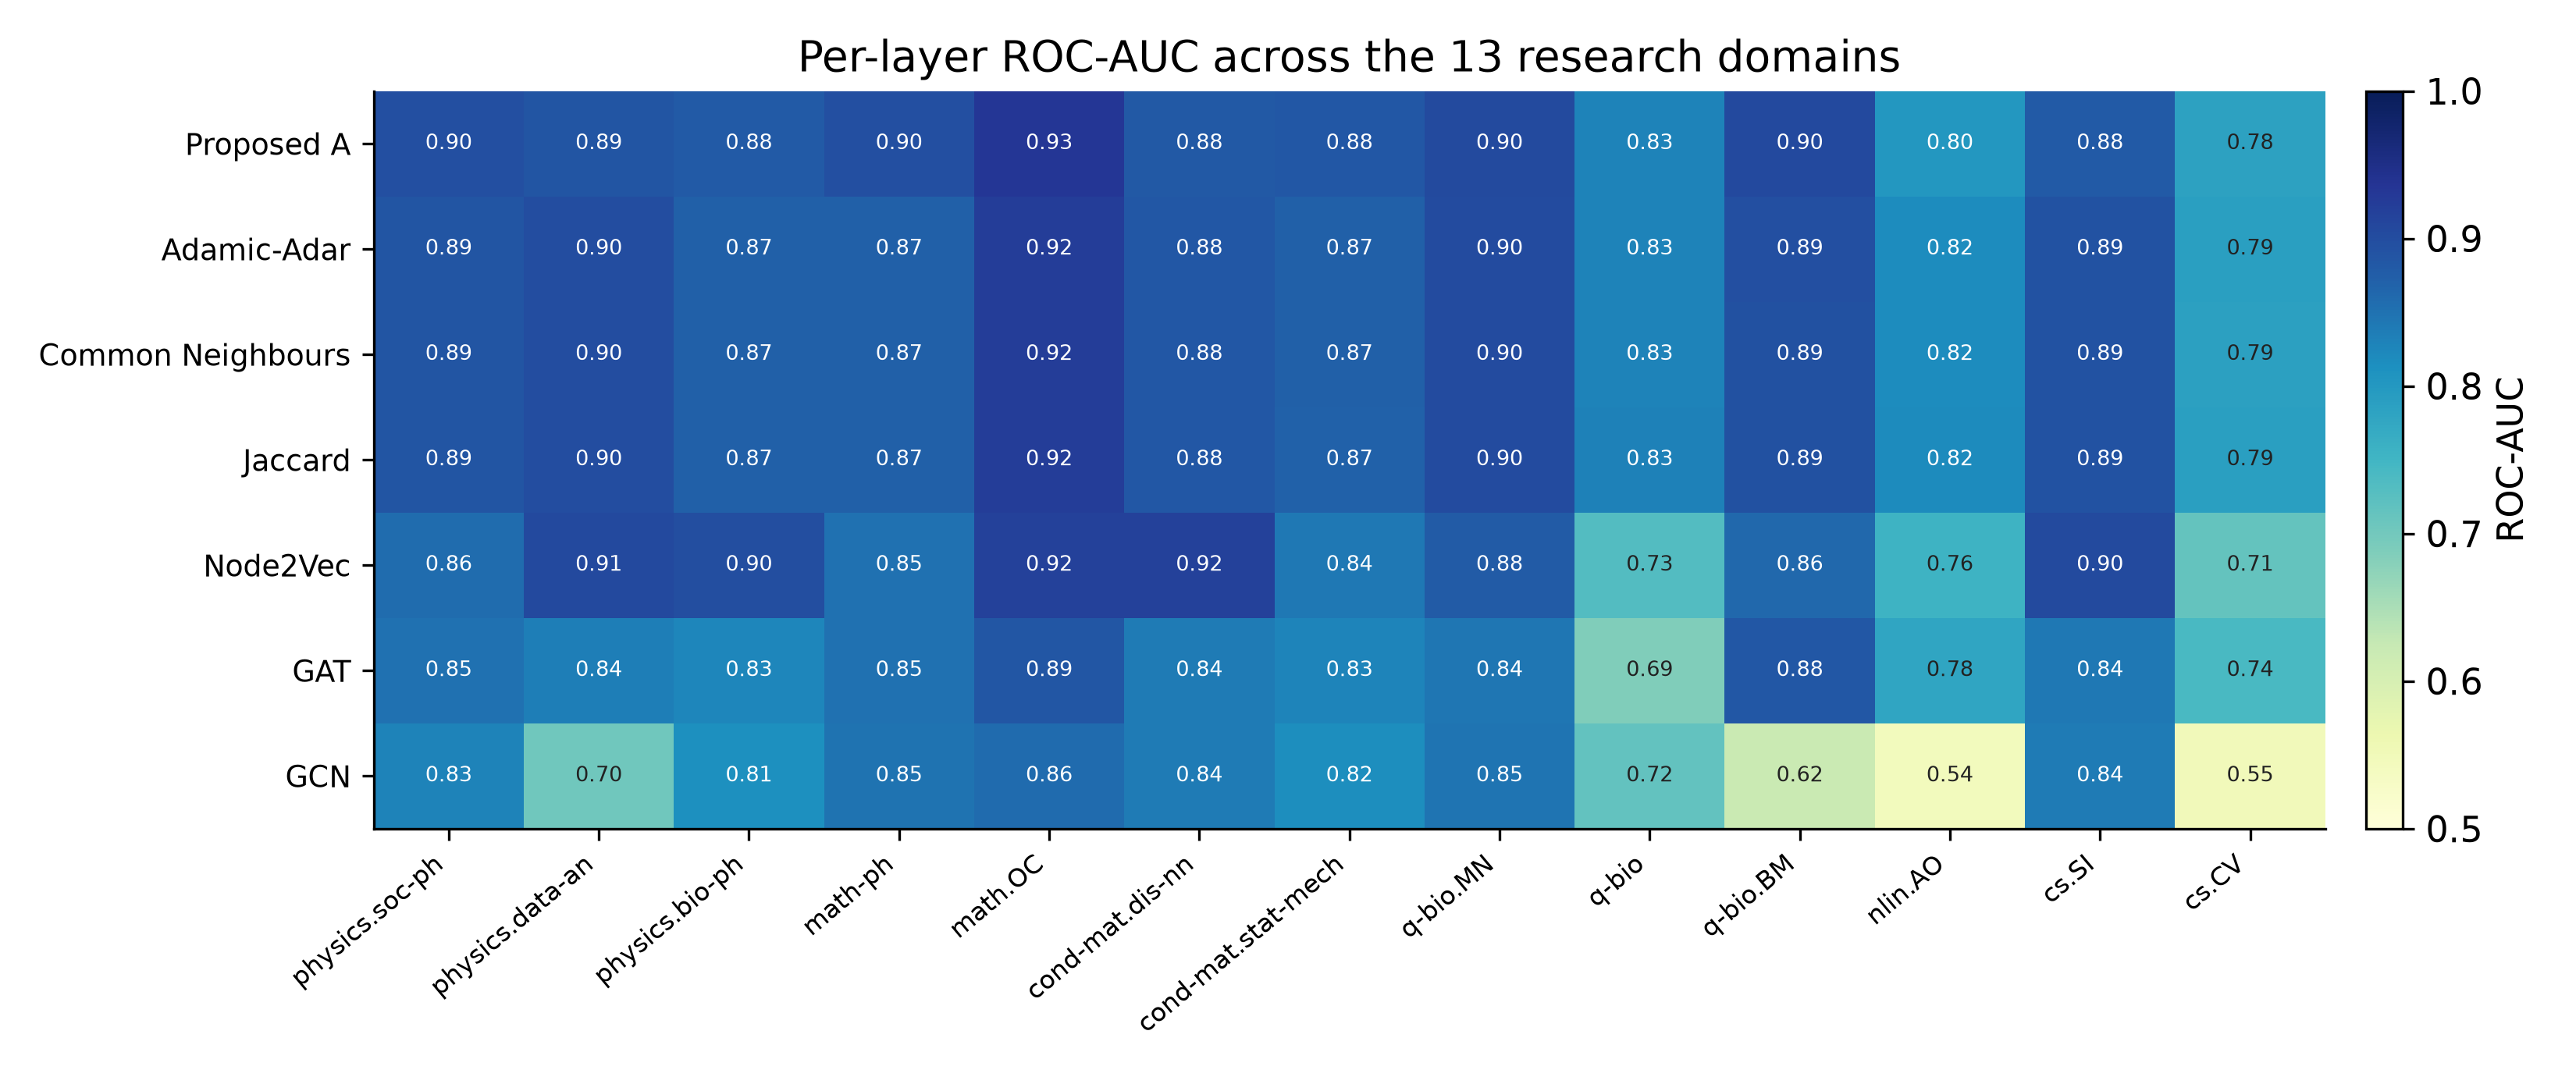
\includegraphics[width=0.98\textwidth]{figures/fig4_per_layer_heatmap.png}
\caption{Per-layer ROC-AUC across the 13 research domains for the main methods.}
\label{fig:heatmap}
\end{figure}

\begin{figure}[htbp]
\centering
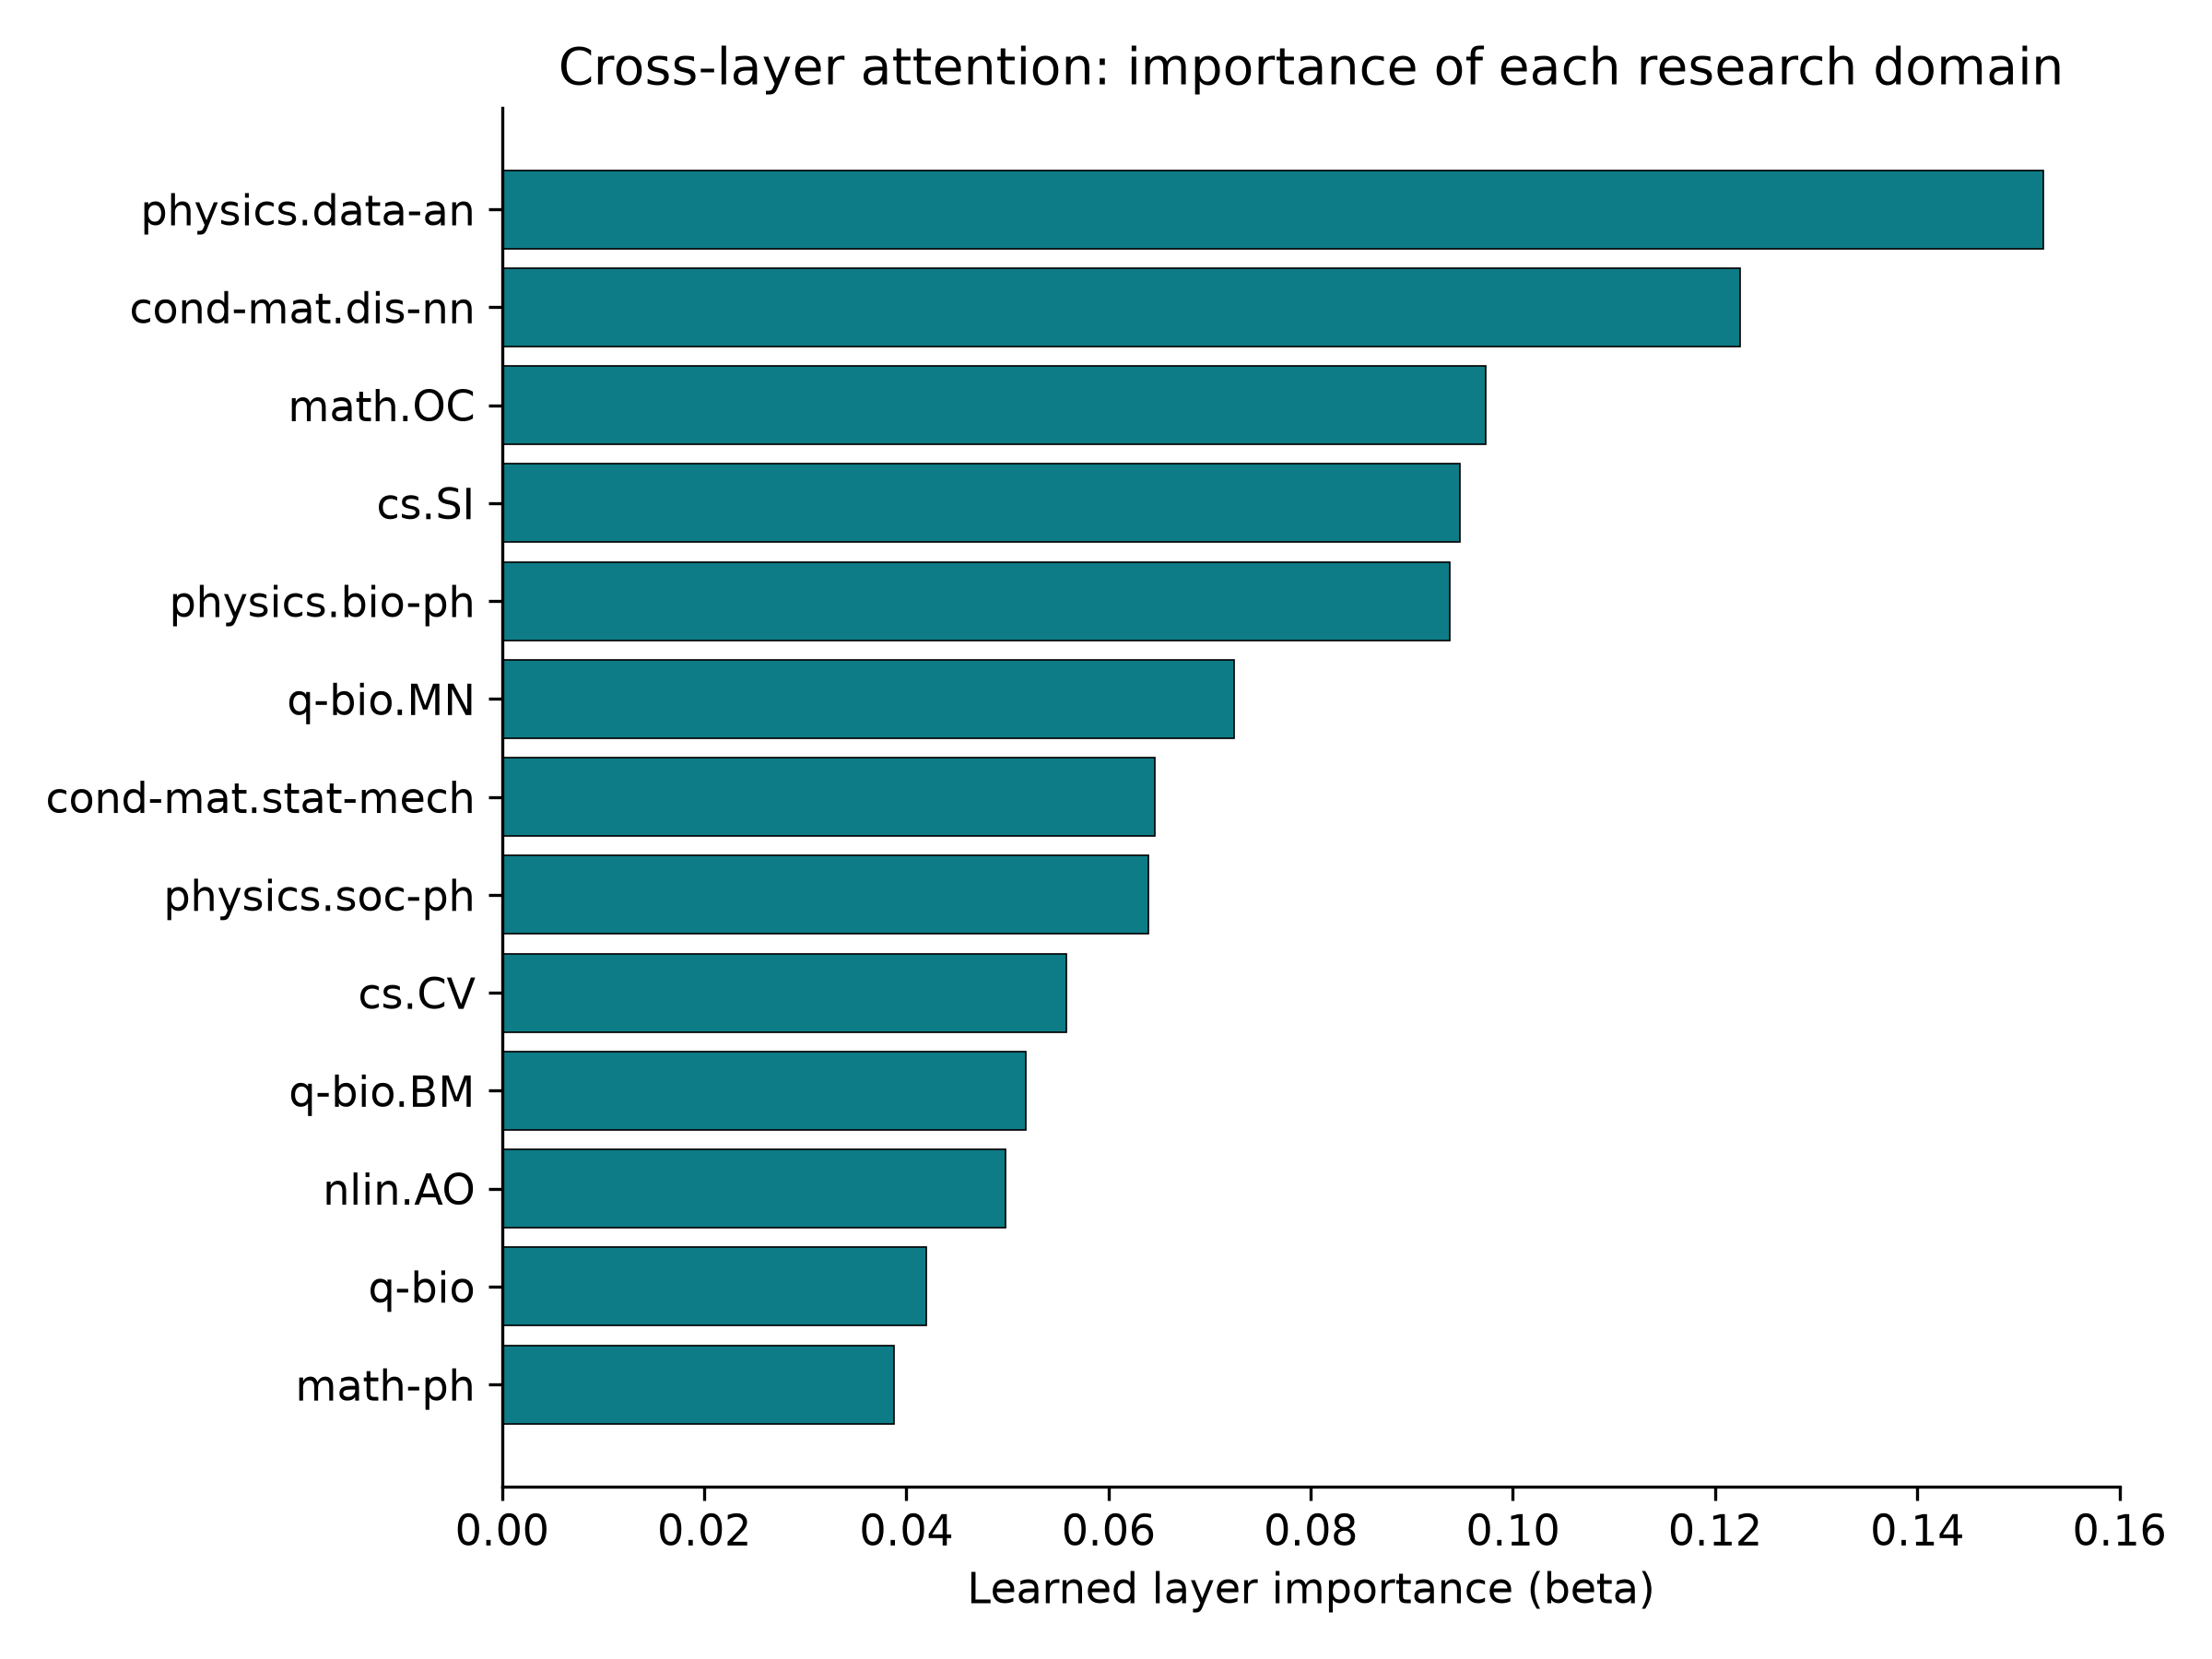
\includegraphics[width=0.75\textwidth]{figures/fig5_layer_importance.png}
\caption{Learned cross-layer attention weights ($\beta$): the importance the model assigns to each
research domain.}
\label{fig:beta}
\end{figure}

\section{Discussion}
Taken together, the results support a nuanced but honest conclusion. The proposed model is
\textbf{not} uniformly the best method: classical heuristics beat it on common-neighbour links and on
ranking, and Node2Vec beats it on PR-AUC and F1. Its contribution is threefold and specific. First,
it achieves the \textbf{best overall ROC-AUC} and a \emph{statistically significant} improvement over
the graph-neural baselines it directly extends. Second, it is the \textbf{best all-rounder} on the
weak-tie/common-neighbour split -- the only method that handles both link types, where every classical
method is provably random on weak ties. Third, it is \textbf{interpretable} through its cross-layer
attention weights. The weak-tie signal and the cross-layer attention are therefore justified not by a
clean sweep of every metric, but by giving the model a capability -- predicting bridging links, with
an explanation -- that the strong-on-average baselines structurally lack.
